%%% The BEGINNING ~~~~~
%%
% ~ Writes FPG--SI | By Filipe G. Vieira & George Pacheco.

%% Preamble Settings %%

% Defines document class and paper size ~
\documentclass[twoside, british, a4paper]{article}
\usepackage[paper=portrait, pagesize]{typearea}

\usepackage{amsmath}
\usepackage{amsfonts}
\usepackage{amssymb,upref}
\usepackage{tgheros}
\usepackage{tgtermes}
\usepackage{anyfontsize}
\usepackage{enumitem}
\usepackage{siunitx}
\usepackage{balance}
\usepackage{float}
\usepackage{pdflscape}
\usepackage[nottoc]{tocbibind}

\usepackage{subfigure}
\usepackage[subfigure]{tocloft}
\setlength\cftbeforefigskip{20pt}
\cftsetindents{fig}{0pt}{0pt}

% Fixes margins ~
\usepackage{geometry}
\geometry{reset, ignoreall,
  textheight = 253mm,
  textwidth = 175mm,
  bottom = 21mm,
  inner = 17.5mm,
  footskip = 8mm,
  headsep = 5mm,
  headheight = 10pt}
\usepackage[utf8]{inputenc}
\usepackage{fancyhdr}
\renewcommand{\headrule}{}
\renewcommand{\footrule}{}

\setlength{\skip\footins}{1.75pc plus 5pt minus 2pt}
\def\footnoterule{
\kern-3mm \hrule height .5pt \kern -.4pt 
\kern 1mm}

\pagestyle{fancy}
\fancyhead[L]{Feral Pigeon Genomics}
\fancyhead[R]{Pacheco et al. 2022}
\fancypagestyle{firstpage}{%
\fancyhf{}
\lhead{}
\rhead{}}


\fancypagestyle{mylandscape}{
\fancyhf{} %Clears the header/footer
\fancyfoot{% Footer
\makebox[\textwidth][r]{% Right
  \rlap{\hspace{.75cm}% Push out of margin by \footskip
    \smash{% Remove vertical height
      \raisebox{4.87in}{% Raise vertically
        \rotatebox{90}{\thepage}}}}}}% Rotate counter-clockwise
\renewcommand{\headrulewidth}{0pt}% No header rule
\renewcommand{\footrulewidth}{0pt}% No footer rule
}

% Loads packages for images ~
\usepackage{graphicx}
\usepackage{rotating}

% Loads packages for comments ~
\usepackage{verbatim}
\usepackage[hang, flushmargin]{footmisc}

% Loads packages for tables ~
\usepackage{float}
\usepackage{multirow}
\usepackage{charter}
\usepackage{textcomp}
\usepackage[utf8]{inputenc}
\usepackage[TU]{fontenc}

% Listing of source code ~
\usepackage{listings}
\usepackage{color}
\definecolor{dkgreen}{rgb}{0,0.6,0}
\definecolor{gray}{rgb}{0.5,0.5,0.5}
\definecolor{mauve}{rgb}{0.58,0,0.82}
\lstset{
  frame = tb,
  language = sh,
  aboveskip = 3mm,
  belowskip = 3mm,
  showstringspaces = false,
  columns = flexible,
  basicstyle = {\small\ttfamily},
  numbers = none,
  numberstyle = \tiny\color{gray},
  keywordstyle = \color{blue},
  commentstyle = \color{dkgreen},
  stringstyle = \color{mauve},
  breaklines = true,
  breakatwhitespace = true,
  tabsize = 3}
  
% Changes caption starting text ~
\renewcommand{\listfigurename}{List of Supplementary Figures}
\renewcommand{\figurename}{}
\renewcommand{\tablename}{}

% Loads packages for typing ~
\usepackage{lettrine}
\pdfmapfile{=montserrat.map} 
\renewcommand{\LettrineFont}{
  \fontfamily{iwonal}\fontsize{30}{30}\selectfont
  \color[rgb]{0.25,0.25,0.25}}
\usepackage{marvosym}

\newcommand\myhline{%
  \noindent\rule[.5pt]{\linewidth}{.4pt}\par%
}

\newcommand{\myheaders}[1] {\noindent{\normalsize{\fontfamily{bch}\selectfont{\textbf{#1}}}}}
\newcommand{\mysubheaders}[1] {\noindent{\fontfamily{bch}\selectfont{\textbf{#1}}}}
\newcommand{\mytext}[1] {\noindent{\fontfamily{bch}\selectfont{#1}}}
\newcommand{\mycaptions}[1] {\noindent{\footnotesize{\fontfamily{bch}\selectfont{#1}}}}

% Figure captions
\usepackage{caption}
\DeclareCaptionFont{charter}{\footnotesize{\fontfamily{charter}\selectfont{#1}}}
\DeclareCaptionLabelSeparator{vline}{\;|\;}
\captionsetup{
 labelsep=vline, 
 font={charter}, 
 labelfont={charter},
 belowskip=-12pt}
\newcommand{\figurecaption}[2]{\caption[#1]{\textbf{#1.} #2}}
\usepackage{hyperref}
\usepackage[dvipsnames]{xcolor}
\definecolor{mycolor}{HTML}{F7F8E0}
\definecolor{myorange}{RGB}{245,156,74}
\hypersetup{
  colorlinks = true,
  linkcolor = [RGB]{58, 121, 175},
  urlcolor = -myorange}

\usepackage{fontawesome}

\usepackage[nopar]{lipsum}
\newcommand\blfootnote[1]{%
  \begingroup
  \renewcommand\thefootnote{}\footnote{#1}%
  \addtocounter{footnote}{-1}%
  \endgroup}

% Loads packages for bibliography ~
\usepackage[
backend = biber,
style = nature,
sorting = ynt
]{biblatex}
\addbibresource{FPGP--MainText.bib}

\usepackage{blindtext}
\usepackage{multicol}

%% Starts Document %%

\usepackage{chngcntr}
\counterwithin{figure}{section}  % Adds figure numbering 1.1, 1.2, ..., 2.1 etc. 
\AtBeginDocument{%
\counterwithin{lstlisting}{section}  % Adds figure numbering 1.1, 1.2, ..., 2.1 etc. 
}

% Starts document ~
\begin{document}\thispagestyle{empty}

\hfill\break

% Sets title ~
\Large{\bfseries{\fontfamily{cmr}\color[rgb]{0,0,0}\noindent{SUPPLEMENTARY INFORMATION FOR}}} \\

\hfill
\hfill

% Sets title ~
\LARGE{\bfseries{\fontfamily{cmr}\color[rgb]{0.25,0.25,0.25}\noindent{On the Origin and Spread of Feral Pigeons}}} \\

% Sets authorship ~
\fontfamily{cmr} \small \noindent 
George Pacheco\,$^{1}$\textsuperscript{\faEnvelopeO},
Filipe G. Vieira\,$^{1}$,
Michael D. Martin\,$^{1}$,
Morten Tange Olsen\,$^{1}$,
Pavel Hulva\,$^{1}$,
Tânia de Freitas Raso\,$^{1}$,
Peter Njoroge\,$^{1}$,
Concepción Salaberria\,$^{1}$,
Isabel López-Rull\,$^{1}$,
Carles Lalueza-Fox\,$^{1}$,
Oscar Ramírez\,$^{1}$,
María C. Ávila-Arcos\,$^{1}$,
Patricia Rosas Escobar\,$^{1}$,
Rui Faria\,$^{1}$,
Miguel Carneiro\,$^{1}$,
Graciela Sotelo\,$^{1}$,
Jóhannis Danielsen\,$^{1}$,
Nizar Haddad\,$^{1}$,
Fares Khoury\,$^{1}$,
Roi Dor\,$^{1}$,
Ali Halajian\,$^{1}$,
María Belén Arias\,$^{1}$,
Oliver Krone\,$^{1}$,
Susanne Auls\,$^{1}$,
Sampath S. Seneviratne\,$^{1}$,
Kajanka Mathiaparanam\,$^{1}$,
Michael Bunce\,$^{1}$,
Megan L. Coghlan\,$^{1}$,
Jon Fjeldså\,$^{1}$ \&
M. Thomas P. Gilbert\,$^{1}$\textsuperscript{\faEnvelopeO} \\
\myhline

% Sets affiliations ~
\blfootnote{\scriptsize{\fontfamily{cmr}$^1$Section for Evolutionary Genomics, The GLOBE Institute, Faculty of Health and Medical Sciences, University of Copenhagen, Copenhagen, Denmark. $^1$Natural History Museum of Denmark, University of Copenhagen, Øster Voldgade 5–7, 1350 Copenhagen, Denmark. $^1$NTNU University Museum, Norwegian University of Science and Technology, Trondheim, Norway $^1$Department of Zoology, Charles University, Prague, Czech Republic. $^1$Departamento de Patologia, Faculdade de Medicina Veterinária e Zootecnia, Universidade de São Paulo, São Paulo, Brazil. $^1$Ornithology Section, Department of Zoology, National Museums of Kenya, Nairobi, Kenya. $^1$Centro de Investigación en Ecosistemas, Universidad Nacional Autonoma de Mexico, Michoacan, Mexico. $^1$Departamento de Ecología Evolutiva, Museo Nacional de Ciencias Naturales, Madrid, Spain. $^1$Avian Evolution Node, Department of Zoology and Environment Sciences, University of Colombo, Colombo, Sri Lanka. $^1$Institute of Evolutionary Biology, Universitat Pompeu Fabra, Barcelona, Spain. $^1$Department of Animal and Plant Sciences, University of Sheffield, Sheffield, UK. $^1$Centro de Investigação em Biodiversidade e Recursos Genéticos, Universidade do Porto, Vairão, Portugal. $^1$Institute of Evolutionary Biology, Department of Experimental and Health Sciences, University, Pompeu Fabra, Spain. $^1$Departamento de Biologia, Faculdade de Ciências, Universidade do Porto, Porto, Portugal. $^1$University of the Faroe Islands, Tórshavn, Faroe Islands. $^1$National Center for Agricultural Research and Extension, Al-Baqah, Jordan. $^1$Department of Biology and Biotechnology, American University of Madaba, Madaba, Jordan. $^1$Department of Zoology, Tel Aviv University, Tel Aviv, Israel. $^1$Natural History Museum, Imperial College of London, London, United Kingdom. $^1$Department of Biodiversity, Turfloop Campus, University of Limpopo, Polokwane, South Africa. $^1$Department of Wildlife Diseases, Leibniz Institute for Zoo and Wildlife Research, Berlin, Germany. $^1$Vetgenomics SL, Edifici Eureka, Campus UAB, Barcelona, Spain. $^1$Trace and Environmental DNA (TrEnD) Laboratory, Department of Environment and Agriculture, Curtin University, Perth, Australia.\\ \textsuperscript{\faEnvelopeO}Correspondence should be addressed to \href{mailto:ganpa@aqua.dtu.dk}{ganpa@aqua.dtu.dk} (G.P.) \& \href{mailto:tgilbert@sund.ku.dk}{tgilbert@sund.ku.dk} (M.T.P.G.)}}

\hfill

\newpage
\clearpage

% Table of Contents %

\clearpage
\pagenumbering{roman}
\let\oldnumberline\numberline
\renewcommand{\numberline}[1]{\oldnumberline{}}
\hfill\break
\listoffigures
\let\numberline\oldnumberline
\newpage

% Suplementary Notes %

\clearpage
\pagenumbering{arabic}
\begin{multicols}{2}
\myheaders{Suplementary Notes} \\
\end{multicols}

\newpage
\clearpage

\begin{landscape}
\thispagestyle{mylandscape}
\begin{figure}
\centering
\includegraphics[width=1.5\textwidth]{../FPG--Pipeline/FPG--Plots/FPG--Stats/FPG--CoverageHeatMap/FPG--CoverageHeatMap.pdf}
\captionsetup{labelformat=empty}
\caption[\textbf{Supplementary Figure 1. Coverage heatmap.}]{\textbf{Supplementary Figure 1. Coverage heatmap.} Columns represent individual samples, while rows represent clusters of loci. Those samples that failed to produce sufficient GBS reads and the blank samples are marked in purple.}
\label{SI:FPG--CovHeatMap}
\end{figure}
\end{landscape}

\begin{figure}
\centering
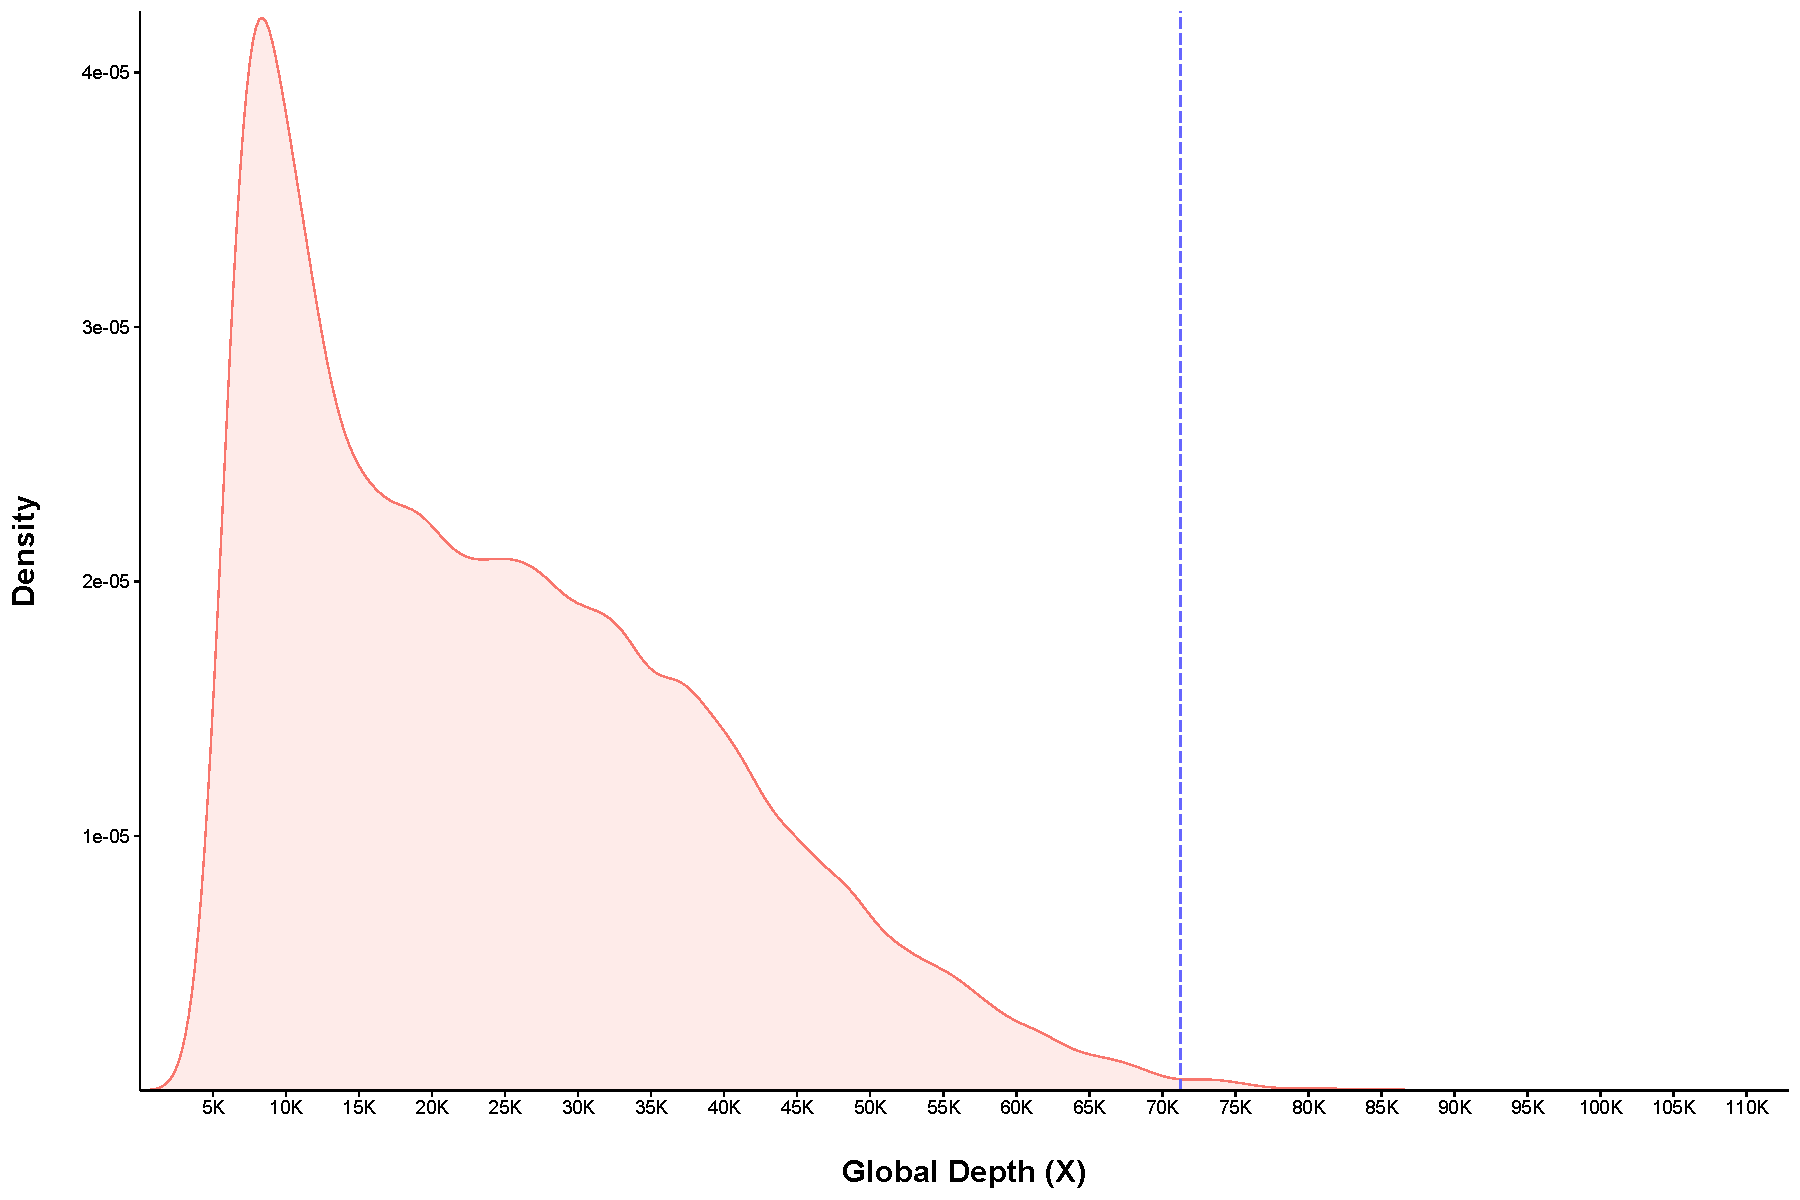
\includegraphics[width=1\textwidth]{../FPG--Pipeline/FPG--Plots/FPG--Stats/FPG--GlobalCoverage/FPG--GlobalCoverage.pdf}
\captionsetup{labelformat=empty}
\caption[\textbf{Supplementary Figure 2. Global Depth (GD) distribution.}]{\textbf{Supplementary Figure 2. Global Depth (GD) distribution.} Density plot of the Global Depth calculated across 475 samples. The purple vertical dashed line indicates the cutoff used, which was a maximum of 150X times the number of individuals in the specific \textit{ANGSD} run.}
\label{SI:FPG--CovDistribution}
\end{figure}

\newpage
\clearpage

\begin{figure}
\centering
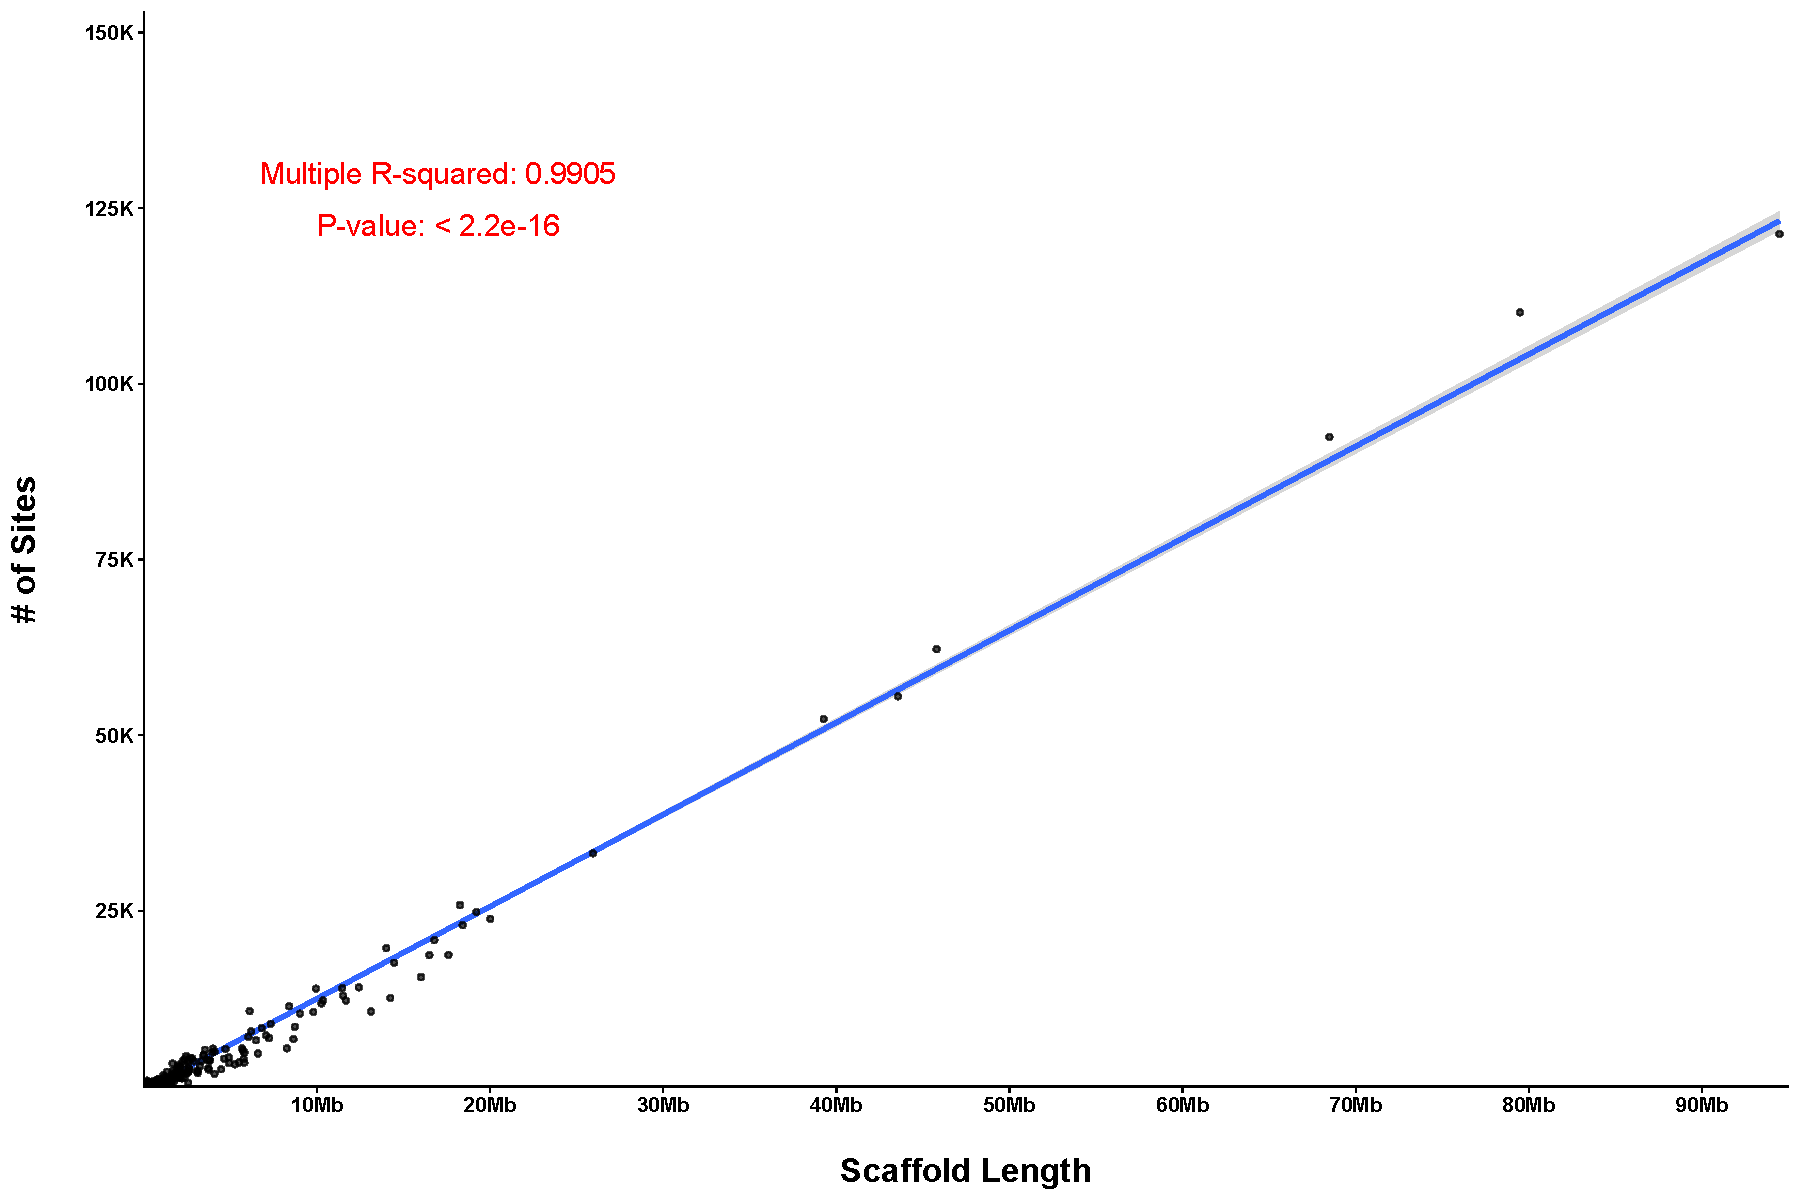
\includegraphics[width=1\textwidth]{../FPG--Pipeline/FPG--Plots/FPG--Stats/FPG--SitesInfo/FPG--Sites-ScaffoldsRegression.pdf}
\captionsetup{labelformat=empty}
\caption[\textbf{Supplementary Figure 3. Scaffold Length Vs Number of Sites regression.}]{\textbf{Supplementary Figure 3. Scaffold Length Vs Number of Sites regression.} Plot of the regression analysis based on Dataset I showing the correlation between the scaffold lengths and numbers of sites found in each scaffold.}
\label{SI:FPG--SitesInfo}
\end{figure}

\begin{figure}
\centering
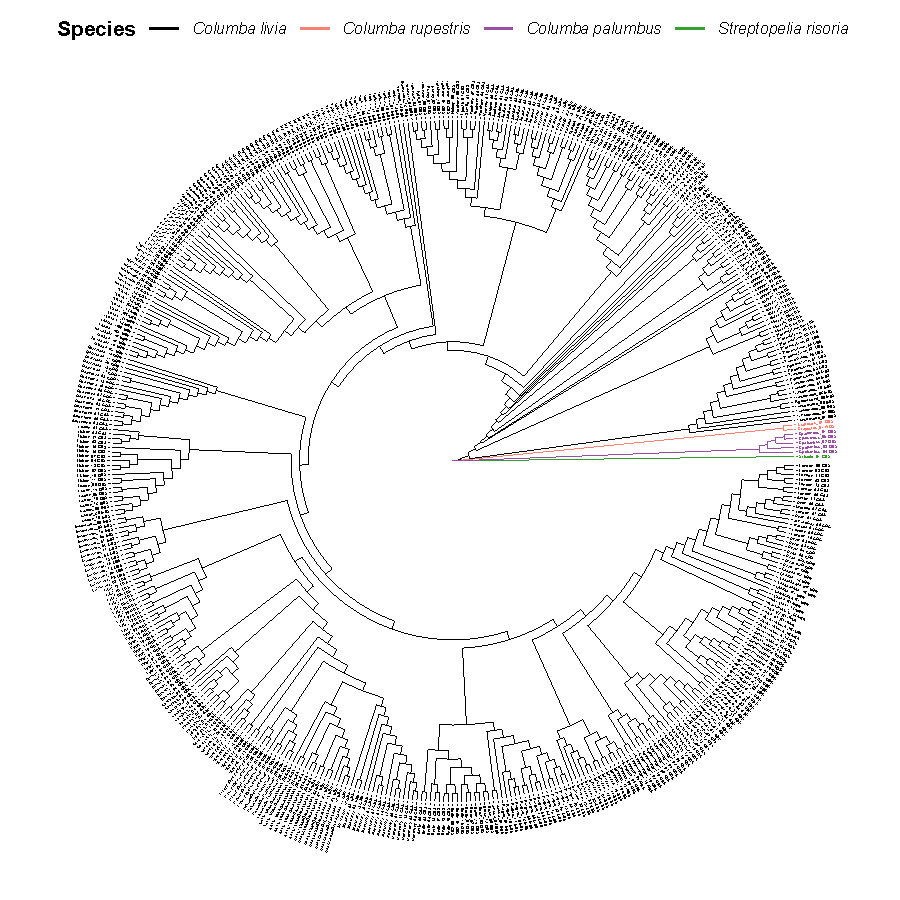
\includegraphics[width=1\textwidth]{../FPG--Pipeline/FPG--Plots/FPG--Phylogenies/FPG--Phylogeny--Dataset_I.pdf}
\captionsetup{labelformat=empty}
\caption[\textbf{Supplementary Figure 4. Cladogram of initial neighbour-joining phylogeny of pigeons.}]{\textbf{Supplementary Figure 4. Cladogram of initial neighbour-joining phylogeny of pigeons.} Initial phylogeny describing the relationships amongst \textit{Columba livia} (black), \textit{C. rupestris} (red), \textit{C. palumbus} (purple) and \textit{Streptopelia risoria} (green).}
\label{SI:FPG--Phylogeny--Dataset_I}
\end{figure}

\begin{figure}
\centering
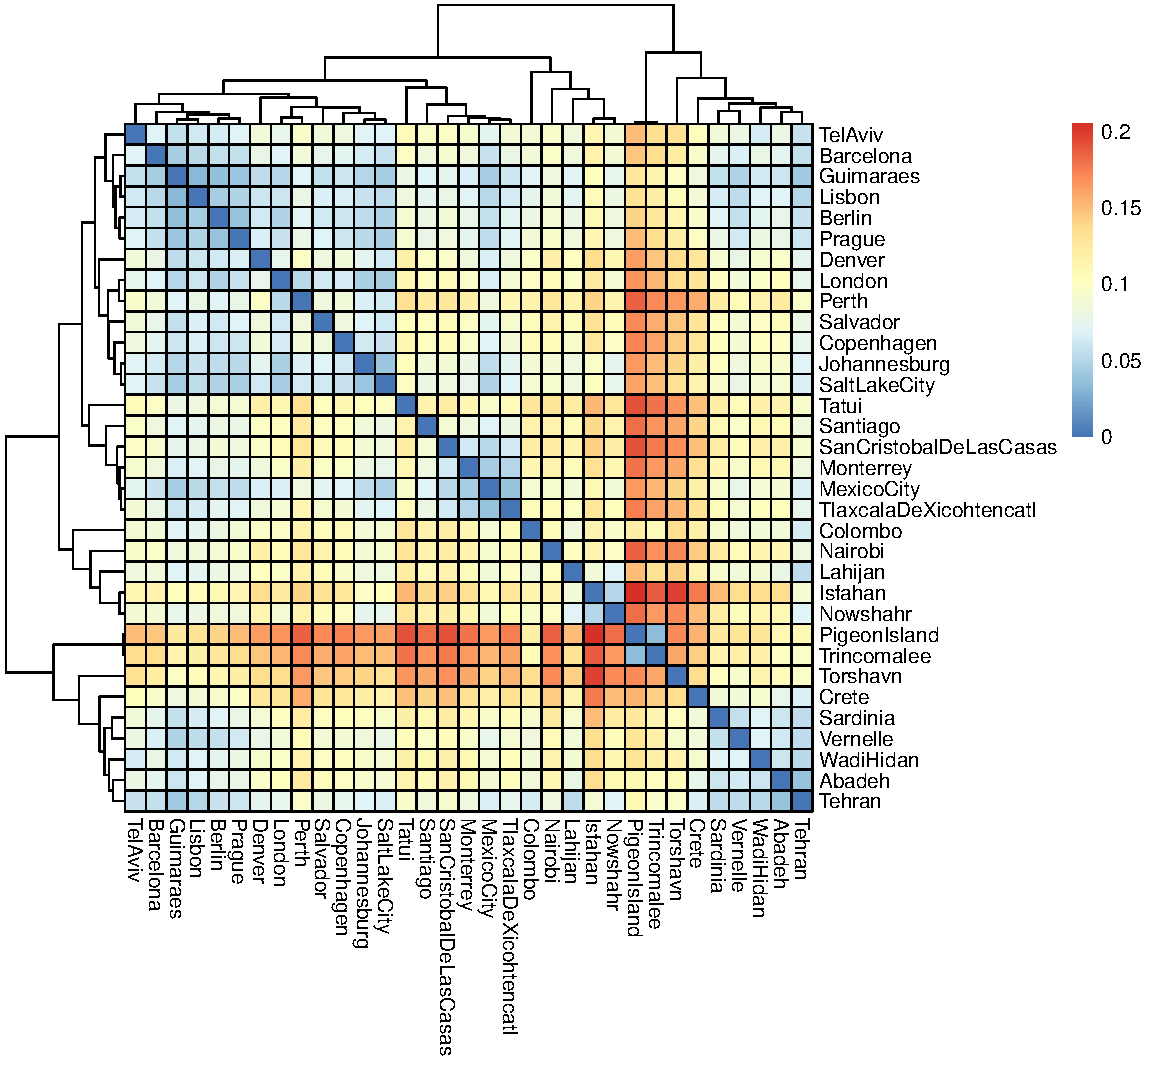
\includegraphics[width=1\textwidth]{../FPG--Pipeline/FPG--Plots/FPG--Fst/FPG--Fst.pdf}
\captionsetup{labelformat=empty}
\caption[\textbf{Supplementary Figure 5. Heatmap of the Pairwise Fst values.}]{\textbf{Supplementary Figure 5. Heatmap of the Pairwise Fst values.} All absolute values can be found in the Supplementary Spreadsheet.}
\label{MainText:FPG--Fst}
\end{figure}

\begin{figure}
\centering
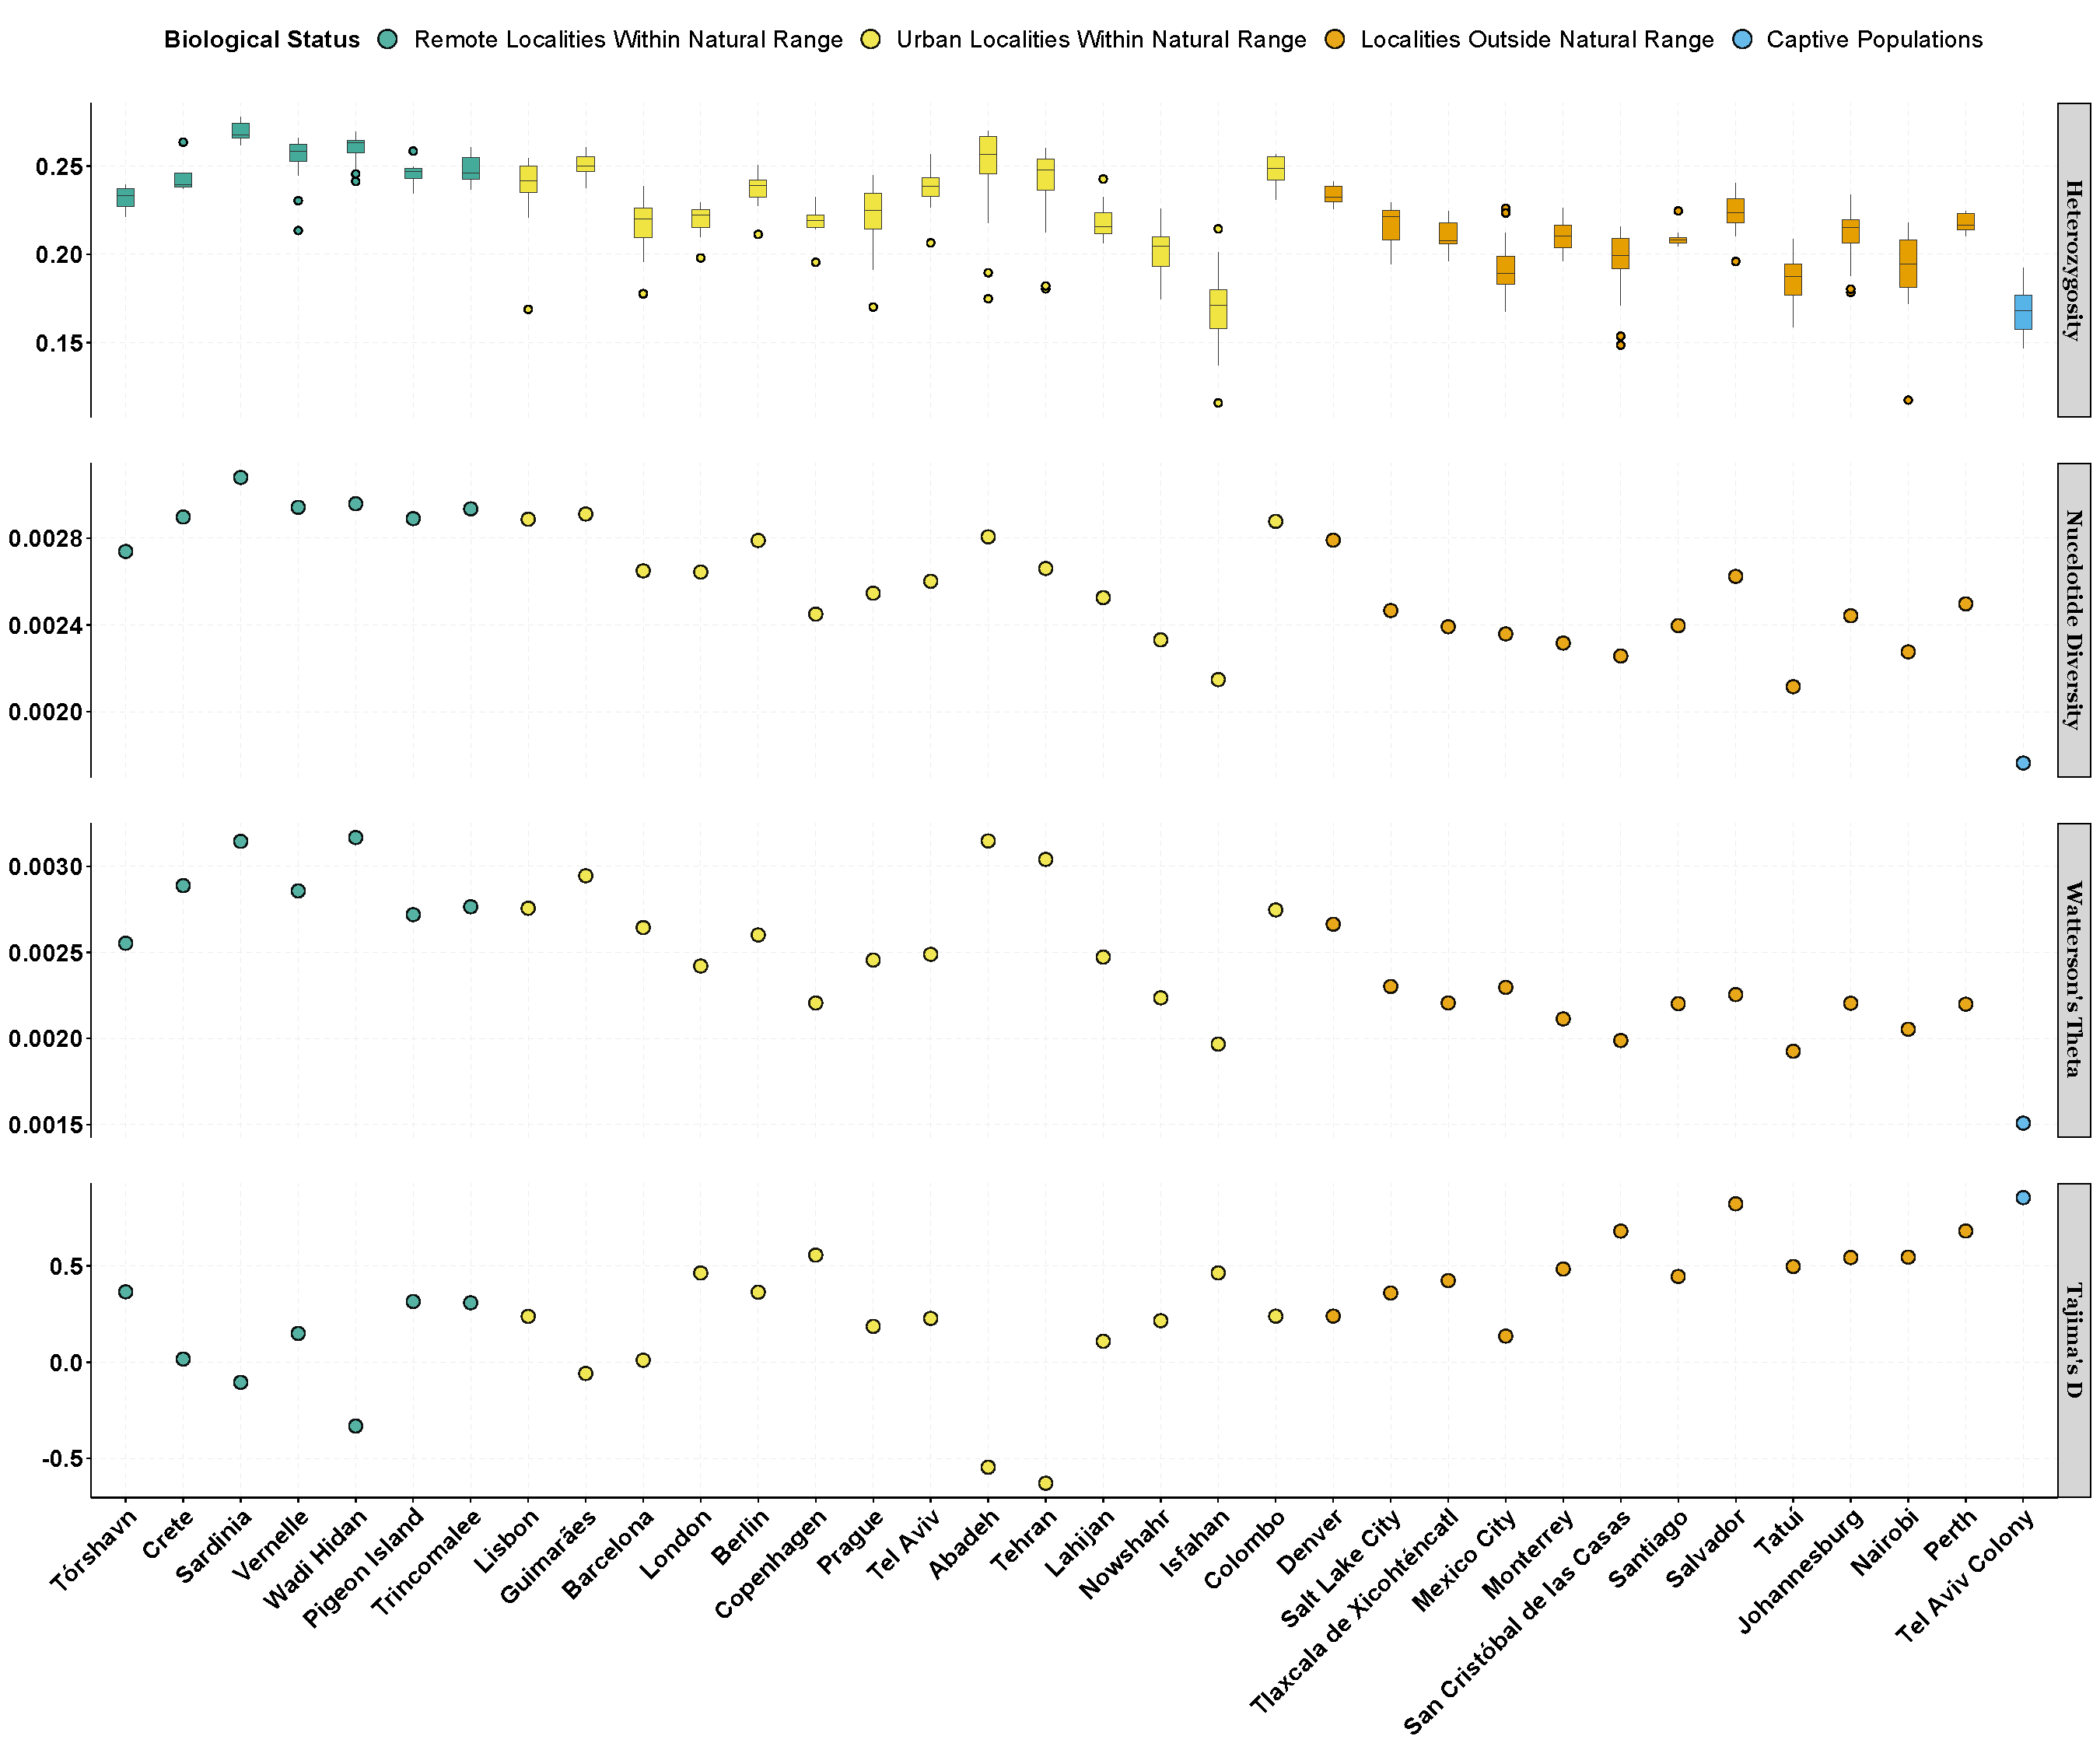
\includegraphics[width=1\textwidth]{../FPG--Pipeline/FPG--Plots/FPG--PopGenEstimates/FPG--PopGenEstimates.pdf}
\captionsetup{labelformat=empty}
\caption[\textbf{Supplementary Figure 6. Population genetics estimates per sampling locality.}]{\textbf{Supplementary Figure 6. Population genetics estimates per sampling locality.} The populations are grouped by the four categories (colours). All absolute values can be found in the Supplementary Spreadsheet.}
\label{MainText:FPG--PopGenEstimates}
\end{figure}

\begin{figure}
\centering
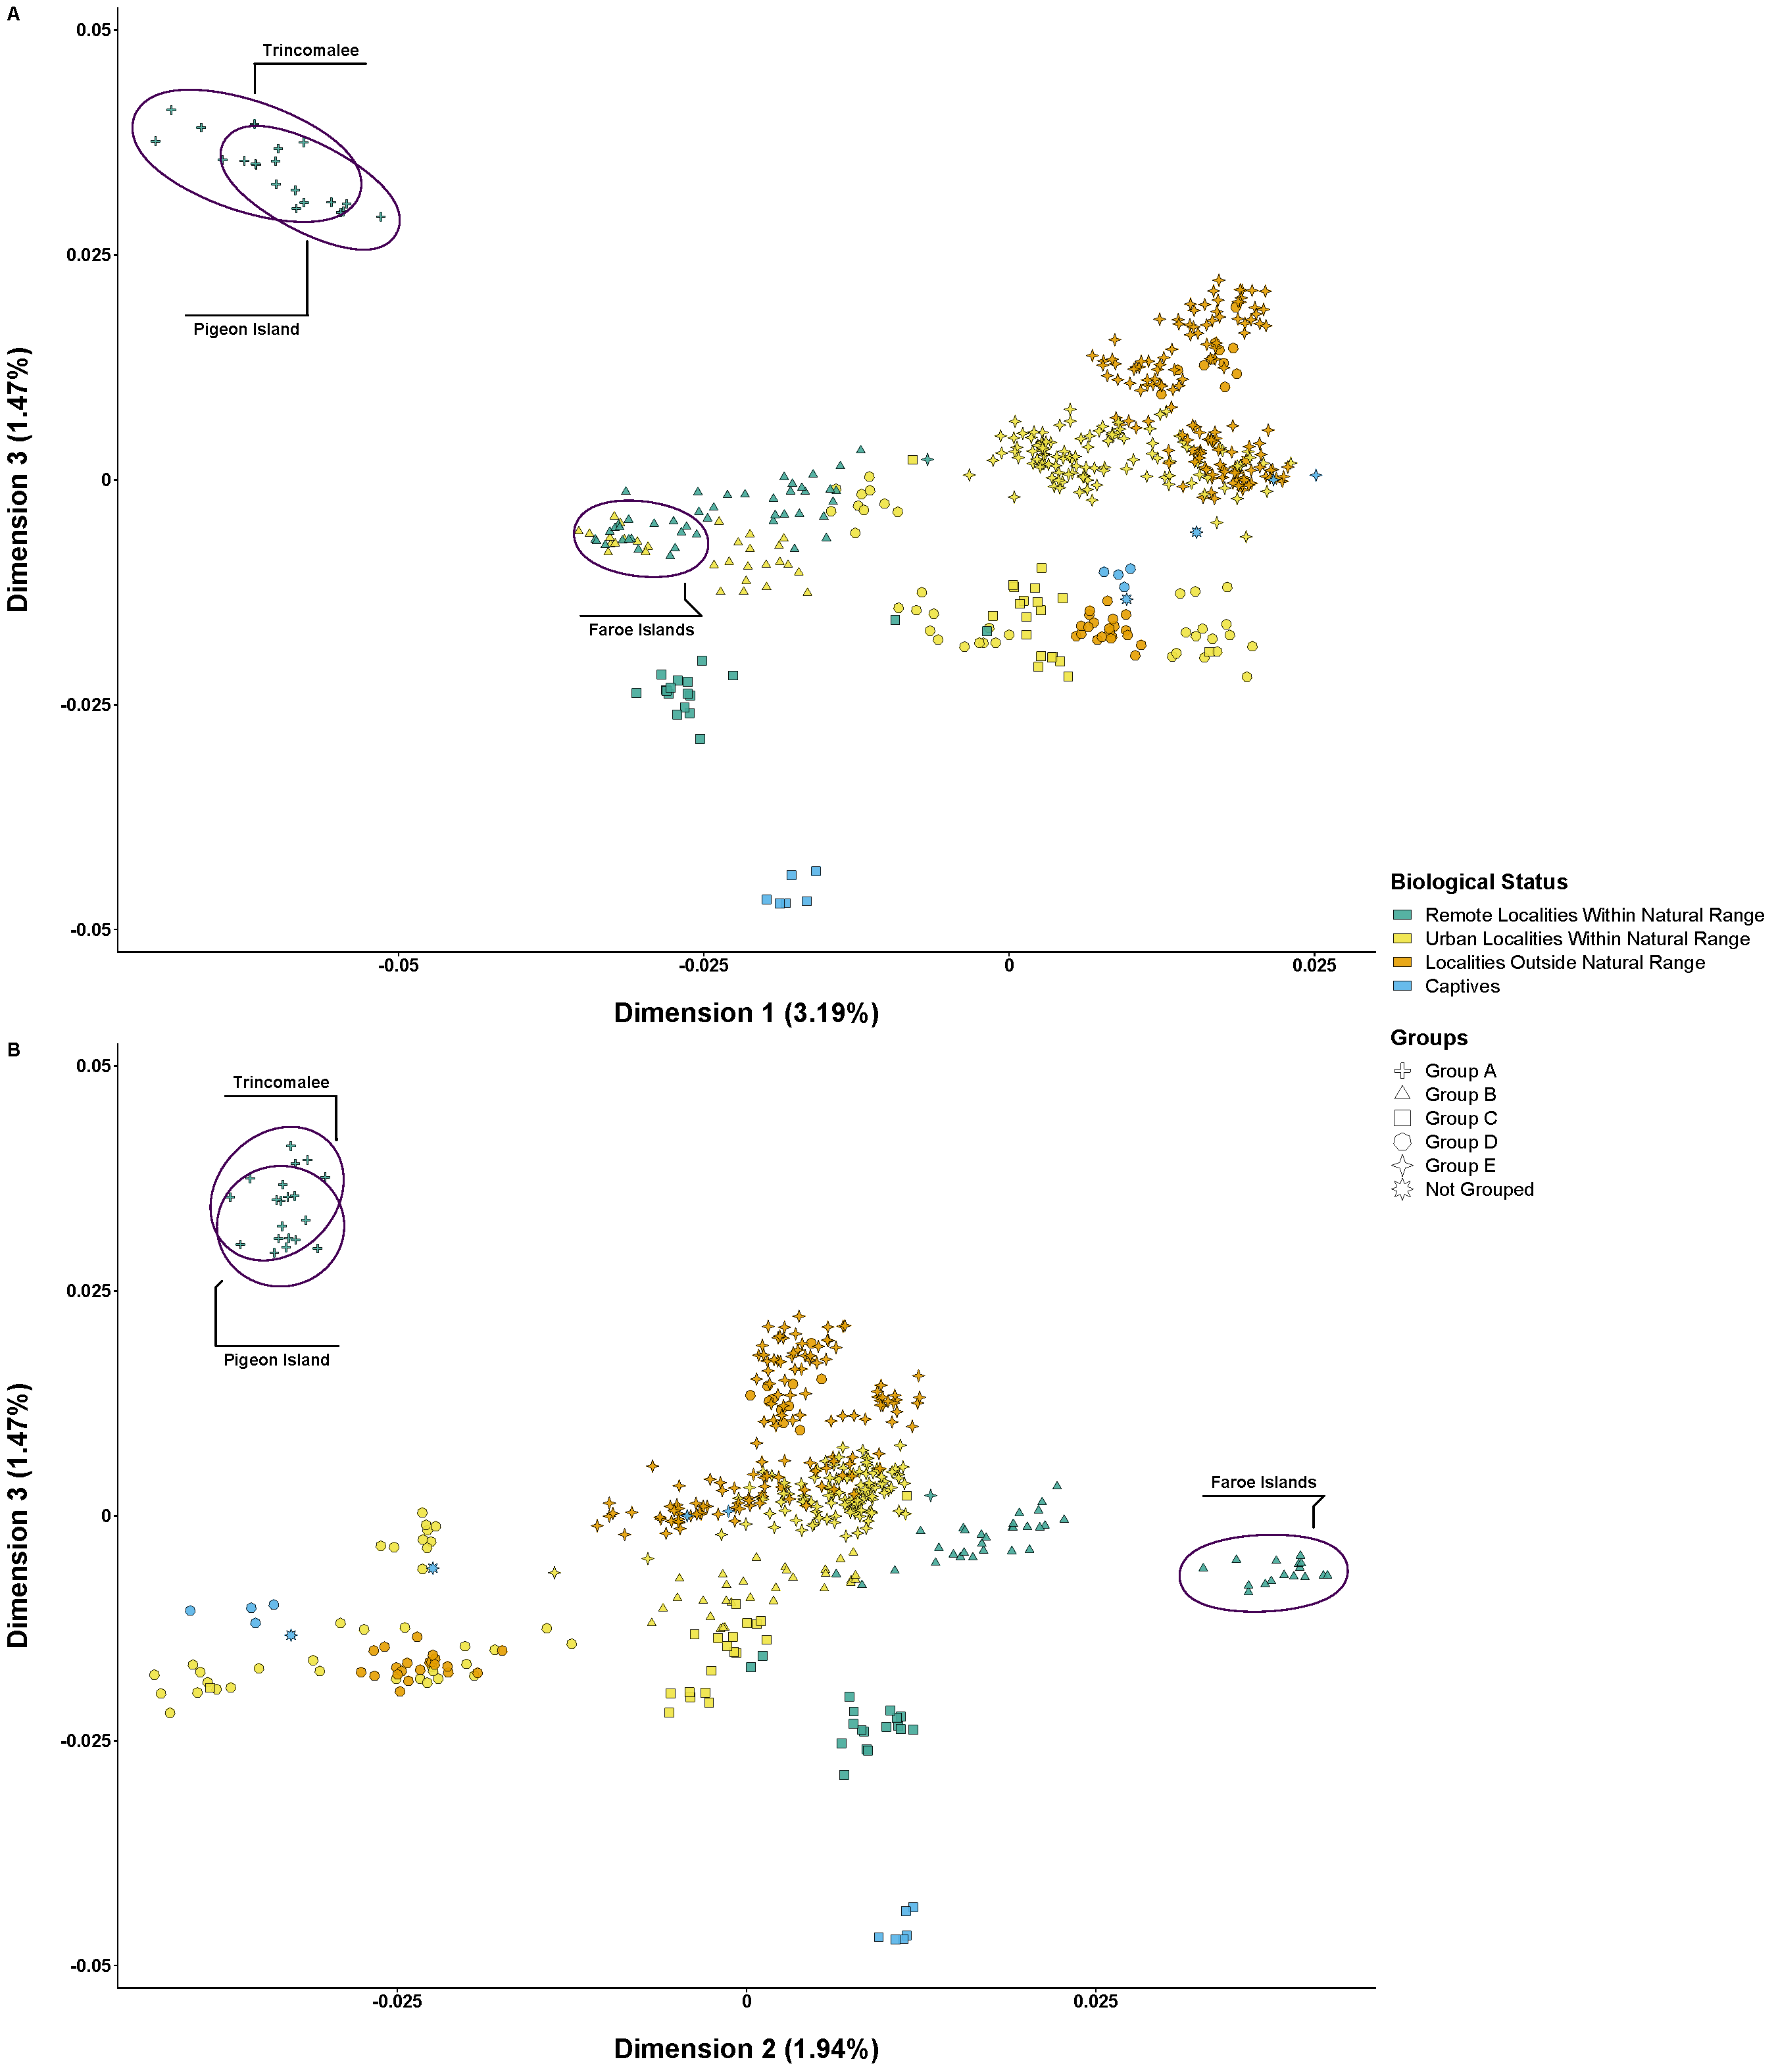
\includegraphics[width=1\textwidth]{../FPG--Pipeline/FPG--Plots/FPG--MDS/FPG--MDS_SI.pdf}
\captionsetup{labelformat=empty}
\caption[\textbf{Supplementary Figure 7. Multidimensional Scaling analysis.}]{\textbf{Supplementary Figure 7. Multidimensional Scaling analysis.} \textbf{A)} Dimensions 1 and 2 are plotted. \textbf{B)} Dimensions 2 and 3 are plotted. Each point on the plot represent a single individual. Individuals are grouped by the four categories (colours), and also by the groups defined in the phylogeny (shapes).}
\label{MainText:FPG--MDS_SI}
\end{figure}

\begin{landscape}
\thispagestyle{mylandscape}
\begin{figure}
\centering
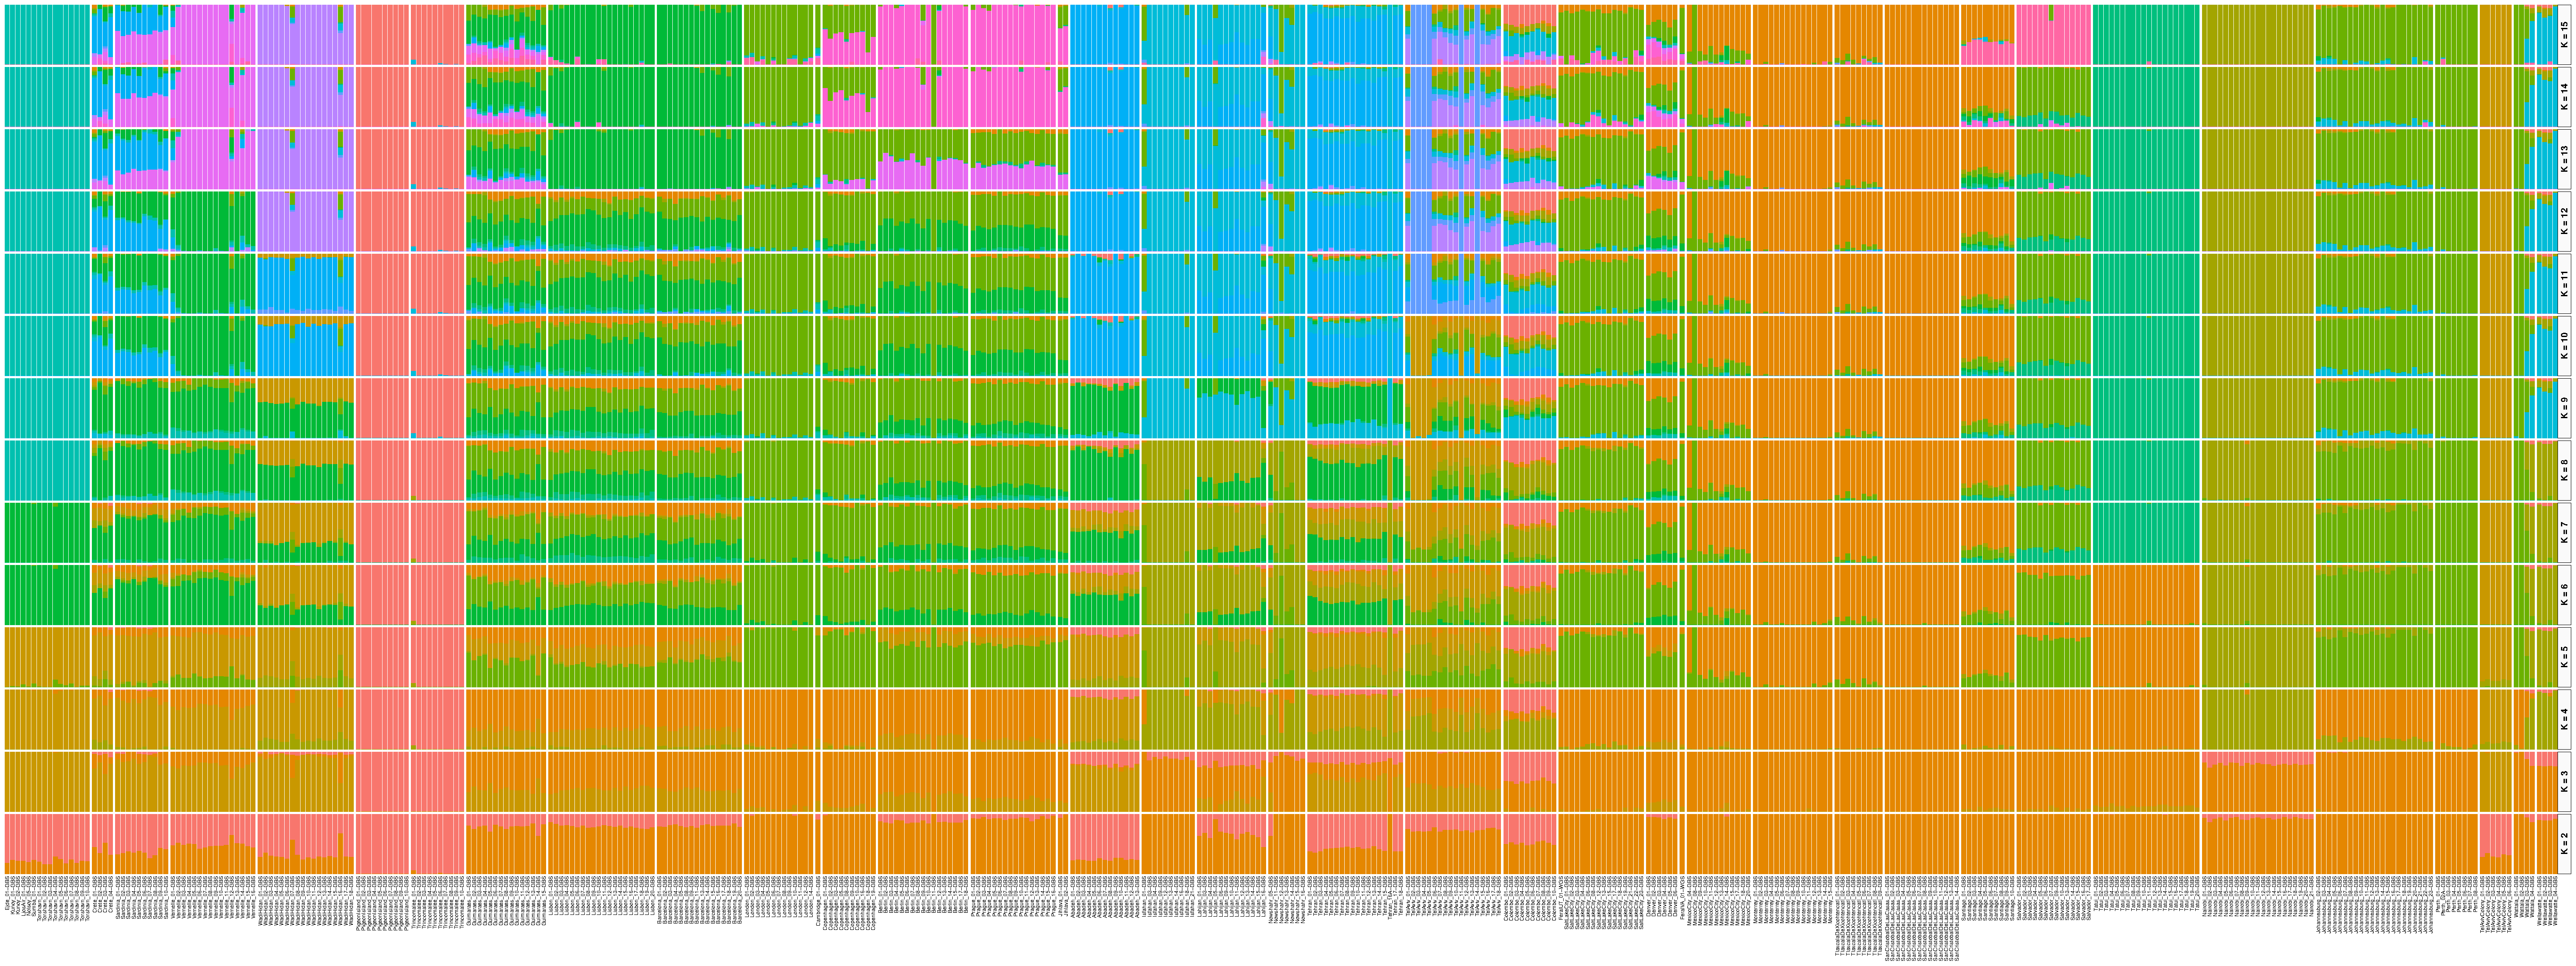
\includegraphics[width=1.5\textwidth]{../FPG--Pipeline/FPG--Plots/FPG--ngsAdmix/FPG--ngsAdmix_Labels-RColours.pdf}
\captionsetup{labelformat=empty}
\caption[\textbf{Supplementary Figure 8. Estimation of Admixture proportions.}]{\textbf{Supplementary Figure 8. Estimation of Admixture proportions.} Individuals are represented by columns, while rows depict the Admixture proportions based on the assumption of different numbers of ancestral populations (K = 2 - 15). This is the same plot presented in the main text but here with the individual labels for all samples.}
\label{MainText:FPG--ngsAdmix_Labels}
\end{figure}
\end{landscape}

\end{document}

% 
%%
%%% The END ~~~~~